\documentclass[../main.tex]{subfiles}

\begin{document}
  \onecolumn

  \clearpage
  \section{プロセッサのブロック図} \label{appendix:block-diagram}
  \begin{figure}[h!]
    \centering
    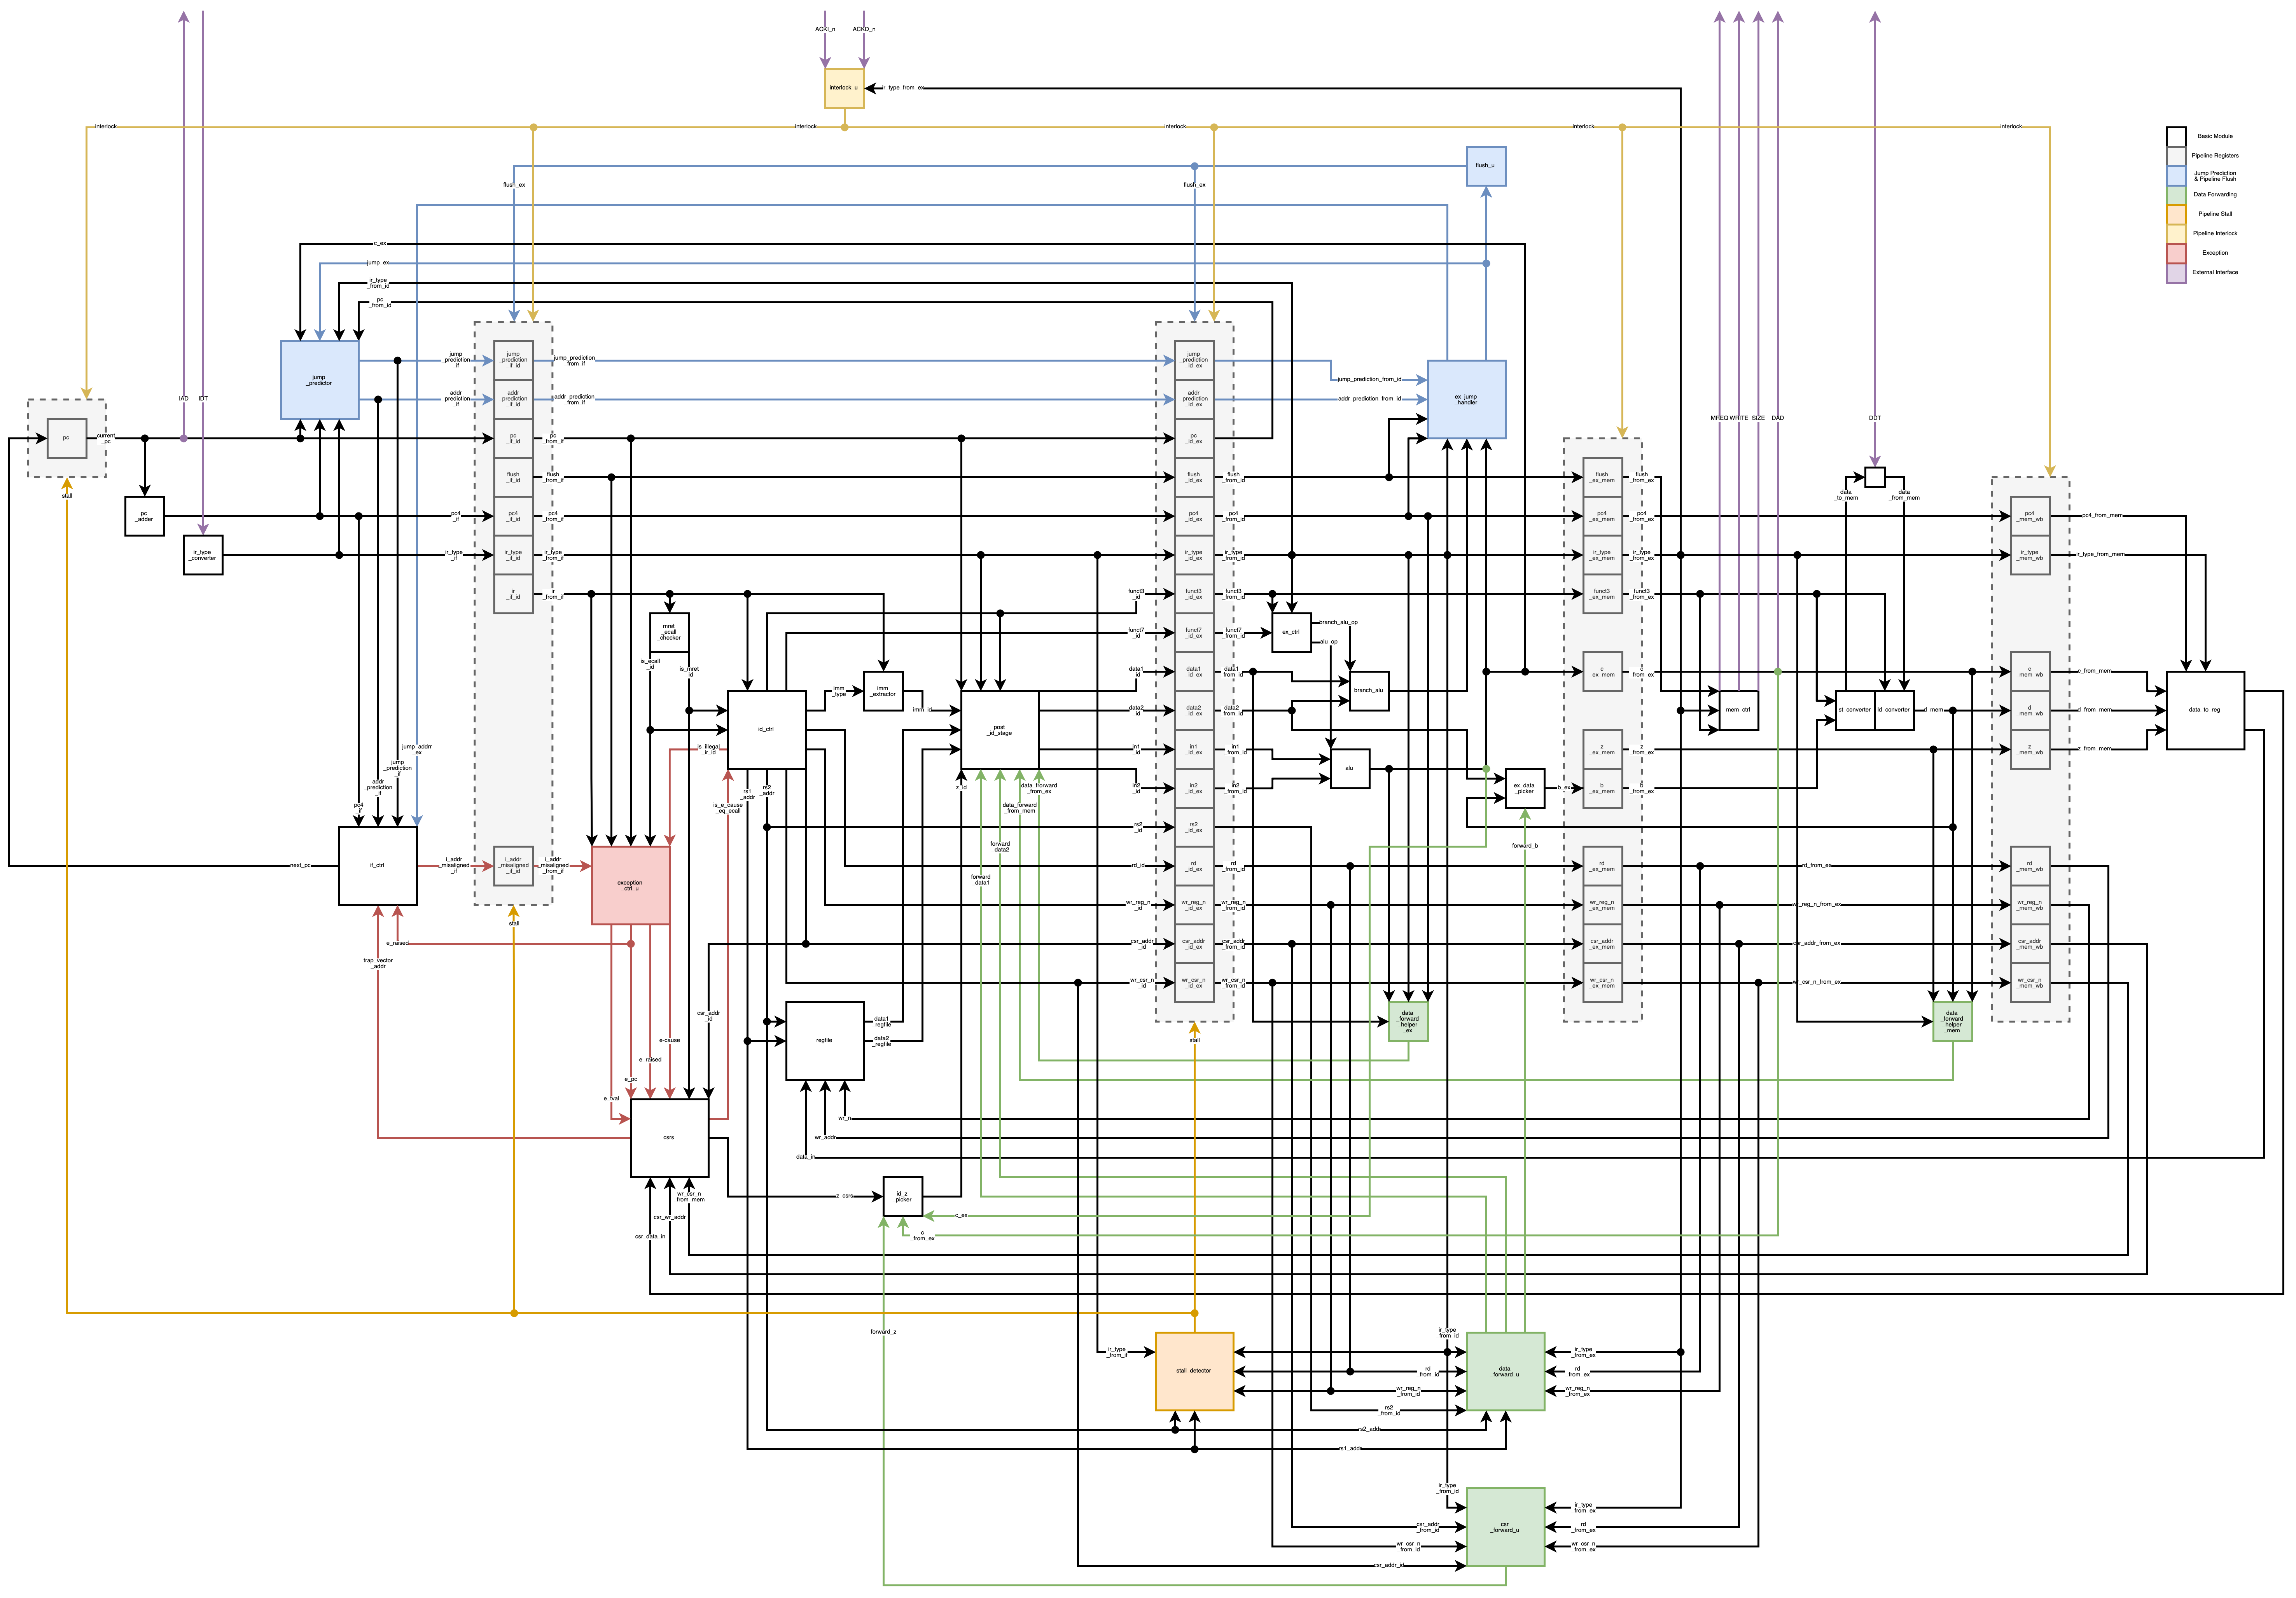
\includegraphics[angle=90, origin=c, totalheight=0.9\textheight]{images/block_diagram.png}
    \caption{プロセッサのブロック図}
    \label{fig:block-diagram}
  \end{figure}

  \clearpage
  \section{サポートしている命令セット} \label{appendix:isa}
  \begin{table*}[h]
    \begin{tabular}{|l|l|l|llll}
    \cline{1-3} \cline{5-7}
    命令    & 内容                                    & 形式 & \multicolumn{1}{l|}{} & \multicolumn{1}{l|}{命令}     & \multicolumn{1}{l|}{内容}                            & \multicolumn{1}{l|}{形式} \\ \cline{1-3} \cline{5-7}
    lui   & load upper immediate                  & U  & \multicolumn{1}{l|}{} & \multicolumn{1}{l|}{add}    & \multicolumn{1}{l|}{add}                           & \multicolumn{1}{l|}{R}  \\
    auipc & add upper immediate to pc             & U  & \multicolumn{1}{l|}{} & \multicolumn{1}{l|}{sub}    & \multicolumn{1}{l|}{sub}                           & \multicolumn{1}{l|}{R}  \\
    jal   & jump and link                         & J  & \multicolumn{1}{l|}{} & \multicolumn{1}{l|}{sll}    & \multicolumn{1}{l|}{shift left logical}            & \multicolumn{1}{l|}{R}  \\
    jalr  & jump and link register                & J  & \multicolumn{1}{l|}{} & \multicolumn{1}{l|}{slt}    & \multicolumn{1}{l|}{set less than}                 & \multicolumn{1}{l|}{R}  \\
    beq   & branch equal                          & B  & \multicolumn{1}{l|}{} & \multicolumn{1}{l|}{sltu}   & \multicolumn{1}{l|}{set less than unsigned}        & \multicolumn{1}{l|}{R}  \\
    bne   & branch not equal                      & B  & \multicolumn{1}{l|}{} & \multicolumn{1}{l|}{xor}    & \multicolumn{1}{l|}{exclusive or}                  & \multicolumn{1}{l|}{R}  \\
    blt   & branch less than                      & B  & \multicolumn{1}{l|}{} & \multicolumn{1}{l|}{srl}    & \multicolumn{1}{l|}{shift right logical}           & \multicolumn{1}{l|}{R}  \\
    bge   & branch greater than or equal          & B  & \multicolumn{1}{l|}{} & \multicolumn{1}{l|}{sra}    & \multicolumn{1}{l|}{shift right arithmetic}        & \multicolumn{1}{l|}{R}  \\
    bltu  & branch less than unsigned             & B  & \multicolumn{1}{l|}{} & \multicolumn{1}{l|}{or}     & \multicolumn{1}{l|}{or}                            & \multicolumn{1}{l|}{R}  \\
    bgeu  & branch greater than or equal unsigned & B  & \multicolumn{1}{l|}{} & \multicolumn{1}{l|}{and}    & \multicolumn{1}{l|}{and}                           & \multicolumn{1}{l|}{R}  \\
    lb    & load byte                             & I  & \multicolumn{1}{l|}{} & \multicolumn{1}{l|}{ecall}  & \multicolumn{1}{l|}{environment call}              & \multicolumn{1}{l|}{I}  \\
    lh    & load halfword                         & I  & \multicolumn{1}{l|}{} & \multicolumn{1}{l|}{csrrw}  & \multicolumn{1}{l|}{csr read and write}            & \multicolumn{1}{l|}{I}  \\
    lw    & load word                             & I  & \multicolumn{1}{l|}{} & \multicolumn{1}{l|}{csrrs}  & \multicolumn{1}{l|}{csr read and set}              & \multicolumn{1}{l|}{I}  \\
    lbu   & load byte unsigned                    & I  & \multicolumn{1}{l|}{} & \multicolumn{1}{l|}{csrrc}  & \multicolumn{1}{l|}{csr read and clear}            & \multicolumn{1}{l|}{I}  \\
    lhu   & load halfword unsigned                & I  & \multicolumn{1}{l|}{} & \multicolumn{1}{l|}{csrrwi} & \multicolumn{1}{l|}{csr read and write immediate}  & \multicolumn{1}{l|}{I}  \\
    sb    & store byte                            & S  & \multicolumn{1}{l|}{} & \multicolumn{1}{l|}{csrrsi} & \multicolumn{1}{l|}{csr read and set immediate}    & \multicolumn{1}{l|}{I}  \\
    sh    & store halfword                        & S  & \multicolumn{1}{l|}{} & \multicolumn{1}{l|}{csrrci} & \multicolumn{1}{l|}{csr read and clear immediate}  & \multicolumn{1}{l|}{I}  \\
    sw    & store word                            & S  & \multicolumn{1}{l|}{} & \multicolumn{1}{l|}{mret}   & \multicolumn{1}{l|}{machine-mode exception return} & \multicolumn{1}{l|}{R}  \\ \cline{5-7}
    addi  & add immediate                         & I  &                       &                             &                                                    &                         \\
    slti  & set less than immediate               & I  &                       &                             &                                                    &                         \\
    sltiu & set less than immediate unsigned      & I  &                       &                             &                                                    &                         \\
    xori  & exclusive or immediate                & I  &                       &                             &                                                    &                         \\
    ori   & or immediate                          & I  &                       &                             &                                                    &                         \\
    andi  & and immediate                         & I  &                       &                             &                                                    &                         \\
    slli  & shift left logical immediate          & I  &                       &                             &                                                    &                         \\
    srli  & shift right logical immediate         & I  &                       &                             &                                                    &                         \\
    srai  & shift right arithmetic immediate      & I  &                       &                             &                                                    &                         \\ \cline{1-3}
    \end{tabular}
    \caption{命令セット}
    \label{table:isa}
  \end{table*}  

  \clearpage
  \section{機能検証と性能評価用プログラム} \label{appendix:programs}
  \begin{table*}[tbh]
    \centering
    \begin{tabular}{|c|c|l|}
    \hline
    テストプログラム & 言語 & プログラム内容 \\ \hline
    load & アセンブリ & ロード命令の動作検証 \\
    store & アセンブリ & ストア命令の動作検証 \\
    p2 & アセンブリ & 演算と分岐命令の動作検証 \\
    trap & アセンブリ & 命令の動作検証 \\
    hello & C & Hello World! をコンソールに表示するプログラム \\
    napier & C & Napier's Constant, $e$ の値を64桁の精度で計算するプログラム \\
    pi & C & pi の値を64桁の精度で計算するプログラム \\
    prime & C & 2を含め, 40個の素数を昇順に見つけるプログラム \\
    bubblesort & C & 100個の整数を Bubble Sort でソートするプログラム \\
    insertsort & C & 100個の整数を Insert Sort でソートするプログラム \\
    quicksort & C & 100個の整数を Quick Sort でソートするプログラム \\ \hline
    \end{tabular}
    \caption{機能検証用プログラム}
    \label{table:test-program}
  \end{table*}

  \begin{table*}[thb]
    \centering
    \begin{tabular}{|c|c|l|}
    \hline
    テストプログラム & 言語 & プログラム内容 \\ \hline
    bitcnts & C & \begin{tabular}[c]{@{}l@{}}7つの方法で与えられた数字の\\ ビット数を求めるプログラム\end{tabular} \\
    stringsearch & C & \begin{tabular}[c]{@{}l@{}}ケース・インセンシティブ方式で\\ 文字の検索するプログラム\end{tabular} \\
    dijkstra & C & \begin{tabular}[c]{@{}l@{}}ダイクストラアルゴリズムで与えられた\\ グラフのノード間の最短距離を求めるプログラム\end{tabular} \\ \hline
    \end{tabular}
    \caption{性能評価用プログラム}
    \label{table:mibench-program}
  \end{table*}
  
\end{document}
